\documentclass[ignorenonframetext, professionalfonts, hyperref={pdftex, unicode}]{beamer}

\usetheme{Belarus}
%\usecolortheme{wolverine}

%Packages to be included
%\usepackage{graphicx}

\usepackage[russian]{babel}
\usepackage[utf8]{inputenc}
\usepackage[T1]{fontenc}

%\usepackage[orientation=landscape, size=custom, width=16, height=9.75, scale=0.5]{beamerposter}

\usepackage{textcomp}

\usepackage{beamerthemesplit}

\usepackage{ulem}

\usepackage{verbatim}

\usepackage{ucs}


\usepackage{listings}
\lstloadlanguages{bash}

\lstset{escapechar=`,
	extendedchars=false,
	language=sh,
	frame=single,
	tabsize=2, 
	columns=fullflexible, 
%	basicstyle=\scriptsize,
	keywordstyle=\color{blue}, 
	commentstyle=\itshape\color{brown},
%	identifierstyle=\ttfamily, 
	stringstyle=\mdseries\color{green}, 
	showstringspaces=false, 
	numbers=left, 
	numberstyle=\tiny, 
	breaklines=true, 
	inputencoding=utf8,
	keepspaces=true,
	morekeywords={u\_short, u\_char, u\_long, in\_addr}
	}

\definecolor{darkgreen}{cmyk}{0.7, 0, 1, 0.5}

\lstdefinelanguage{diff}
{
    morekeywords={+, -},
    sensitive=false,
    morecomment=[l]{//},
    morecomment=[s]{/*}{*/},
    morecomment=[l][\color{darkgreen}]{+},
    morecomment=[l][\color{red}]{-},
    morestring=[b]",
}


\author{Ю.Адамаў, EPAM, Minsk}
\date{23 жніўня 2014}

%\setbeamertemplate{navigation symbols}{}
%\defbeamertemplate*{footline}{decolines theme}{
%  \hbox{
%    \includegraphics[height=0.5cm]{}
%  }
%}


%\institution[EPAM]{EPAM}
%\logo{\includegraphics[width=1cm]{logo.png}}

%\AtBeginSection[]{%
%  \begin{frame}<beamer>
%    \frametitle{}
%    \tableofcontents[
%        sectionstyle=show/shaded, hideallsubsections ]
%  \end{frame}
%  \addtocounter{framenumber}{-1}% If you don't want them to affect the slide number
%}
%
%\AtBeginSubsection[]{%
%  \begin{frame}<beamer>
%    \frametitle{}
%    \tableofcontents[
%        sectionstyle=show/hide,
%        subsectionstyle=show/shaded/hide, ]
%  \end{frame}
%  \addtocounter{framenumber}{-1}% If you don't want them to affect the slide number
%}


\title{Нацыянальна свядомы штучны інтэлект}

\begin{document}
\begin{frame}{}
\titlepage
\end{frame}

\begin{frame}{Што маецца на ўвазе}
\begin{center}
{\Large Think IBM Watson}

Машына, якая можа размаўляць з чалавекам і самастойна збіраць інфармацыю з чалавечых тэкстаў
\end{center}
\begin{itemize}
  \item OCR
  \item Аналіз тэкстаў і збор звестак з іх (NLP)
  \item Пазнаванне чалавечай гаворкі 
  \begin{itemize}
    \item TTS
  \end{itemize}
\end{itemize}
  
\end{frame}

\begin{frame}{}
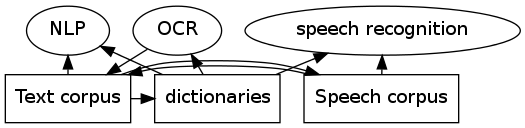
\includegraphics[width=\textwidth]{ai.png}
\end{frame}

\begin{frame}{Рухавікі}
\begin{itemize}
 \item OCR
 \begin{itemize}
  \item cuneiform
  \item tesseract
 \end{itemize}
 \item NLP
 \begin{itemize}
   \item aot?
   \item корпусы
   \item tomita-parser
 \end{itemize}
 \item Гаворка
  \begin{itemize}
   \item CMUSphinx, pocketsphinx
   \item Julius
   \item ...
  \end{itemize}
\end{itemize}
\end{frame}


\begin{frame}{Корпусы тэкстаў}
\begin{itemize}
  \item Ёсць некалькі корпусаў (bnkorpus.info, github.com/poritski/YABC, ...)
  \item Ёсць пытанні з (C)
  \item Ідэі
   \begin{itemize}
     \item crowdsourcing: opencorpora.org engine
     \item Грамадскі набытак: 50 год Шмат класікаў ужо...
   \end{itemize} 
\end{itemize}
\end{frame}

\begin{frame}{Корпусы гаворкі}
  \begin{itemize}
    \item Праект voxforge (nothing/140h)
    \item Праект librivox (1 зборнік вершаў)
  \end{itemize}
\end{frame}

\end{document}
